\documentclass{homework}

\title{Homework 10}
\author{Kevin Evans}
\studentid{11571810}
\date{November 18, 2020}
\setclass{Physics}{341}
\usepackage{amssymb}
\usepackage{mathtools}

\usepackage{amsthm}
\usepackage{amsmath}
\usepackage{slashed}
\usepackage{relsize}
\usepackage{threeparttable}
\usepackage{float}
\usepackage{booktabs}
\usepackage{boldline}
\usepackage{changepage}
\usepackage{physics}
\usepackage[inter-unit-product =\cdot]{siunitx}
\usepackage{setspace}

\usepackage[makeroom]{cancel}
%\usepackage{pgfplots}

\usepackage{enumitem}
\usepackage{times}

\usepackage{calligra}
\DeclareMathAlphabet{\mathcalligra}{T1}{calligra}{m}{n}
\DeclareFontShape{T1}{calligra}{m}{n}{<->s*[2.2]callig15}{}
\newcommand{\scriptr}{\mathcalligra{r}\,}
\newcommand{\boldscriptr}{\pmb{\mathcalligra{r}}\,}

\begin{document}
	\maketitle
	\begin{enumerate}
		\item \begin{enumerate}
			\item It's stationary, as there's no initial velocity and the electric field is zero.
			\item $B=B \uvec{z}$, $v(0) = v_0 \uvec{y}$, the velocity can be written \begin{align*}
				\bvec{v} & = \dot{x} \uvec{x} + \dot{y} \uvec{y} \\
				\bvec{a} & = \ddot{x} \uvec{x} + \ddot{y} \uvec{y}
				\intertext{Balancing the forces,}
				q \bvec{v} \cross \bvec{B} & = m \bvec{\dot{v}} \\
				qB\left(-\dot{x} \uvec{y} + \dot{y} \uvec{x}\right) & = m \left(\ddot{x} \uvec{x} + \ddot{y} \uvec{y}\right)
				\intertext{Equating each compoment, we're left with these coupled equations,}
				-qB \dot{x} & = m \ddot{y} \\
				qB \dot{y} & = m \ddot{x}
				\intertext{Letting $\omega = qB/m$, then letting $u=\dot{x}$,}
				-\omega^2 \dot{x} & = \dddot{x} \\
				-\omega^2 u & = \ddot{u}
				\intertext{The solution for $u(t)$ is sinusoidal and we can integrate to find $x(t)$,}
				u(t) & = A \cos \omega t + B \sin \omega t \\
				x(t) & = C_1 \cos \omega t + C_2 \sin \omega t + C_3
				\intertext{Then for $y$,}
				\ddot{x} & = -C_1 \omega^2 \cos \omega t - C_2 \omega^2 \sin \omega t \\
				\dot{y} & = \frac{ \ddot{x} }{\omega} = -C_1 \omega \cos \omega t - C_2 \omega \sin \omega t \\
				y(t) & = - C_1 \sin \omega t + C_2 \cos \omega t + C_4
				\intertext{For the IC $v(0) = v_0 \uvec{y}$ and assuming the particle starts at $(0, 0)$}
				C_1 & = -\frac{ v_0 }{\omega} \\
				C_2 & = 0 \\
				C_3 & = -C_1 \\
				C_4 & = 0
				\intertext{The equations of motion are}
				x(t) & = \frac{v_0}{\omega} \left(1 - \cos \omega t\right) \\
				y(t) & = \frac{v_0}{\omega} \sin \omega t
			\end{align*}
		% TODO: \usepackage{graphicx} required
		\begin{center}
			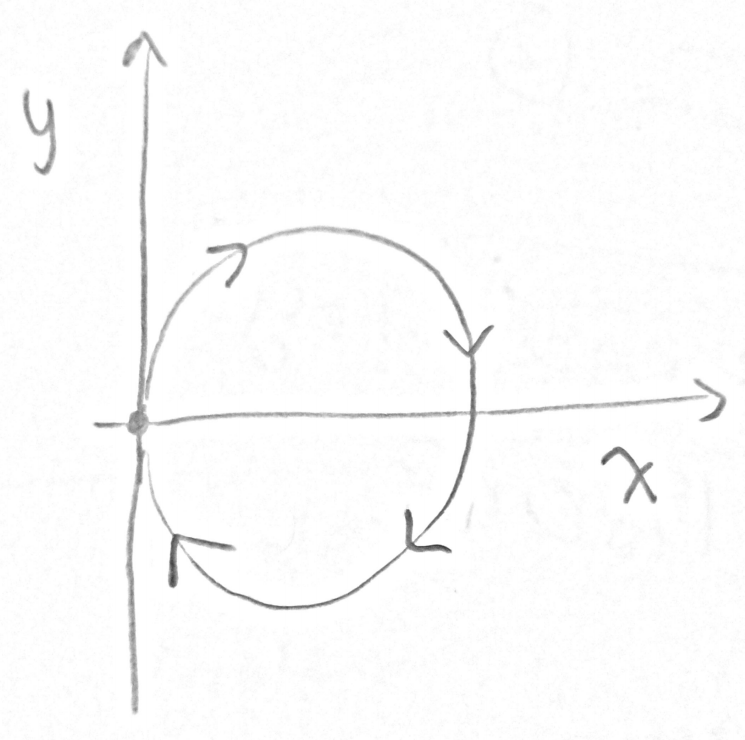
\includegraphics[width=0.5\linewidth]{screenshot001}
		\end{center}
		
			\item Since the velocity is in the direction of the magnetic field and is perpendicular to the electric field, it'll remain constant in the $z$ direction. Taking a similar approach to the Example 5.2 in the book and using (5.7), it's evident that \begin{align*}
				x(t) & = \frac{E}{\omega B} \left(\omega t - \sin \omega t \right) \\
				y(t) & = \frac{E}{\omega B} (1 - \cos \omega t) \\
				z(t) & = \frac{E}{B} t
			\end{align*}
			% TODO: \usepackage{graphicx} required
			\begin{center}
				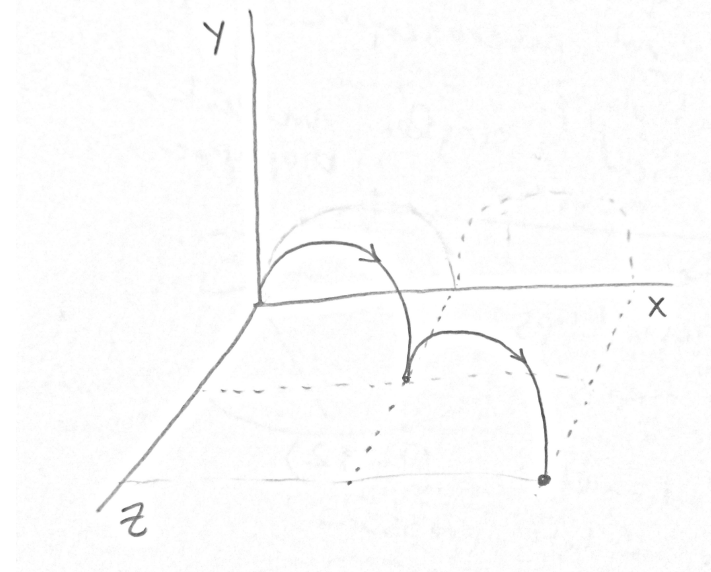
\includegraphics[width=0.5\linewidth]{screenshot002}
			\end{center}
			
			\item Starting from the (b), the electric field would appear in the $y$-force equation as
			$$ qE - qB \dot{x} = m \ddot{y}$$
			and yields \begin{align*}
				\dddot{x} & = \omega^2 \frac{E}{B} - \omega^2 \dot{x} \\
				x(t) & = C_1 \cos \omega t + C_2 \sin \omega t + \frac{E}{B}t + C_3 \\
				y(t) & = -C_1 \sin \omega t + C_2 \cos \omega t + C_4
				\intertext{Using $v(0) = E/B \uvec{x}$ and the particle starting at $(0,0)$, and solving with a $4\cross 5$ matrix,}
				x(t) & = \frac{E}{2B} \left( - \cos \omega t + \sin \omega t + t + 1\right) \\
				y(t) & = \frac{E}{2B} \left(\sin \omega t + \cos \omega t - 1\right)
			\end{align*}
			Pretty sure this one is not right.
			% TODO: \usepackage{graphicx} required
			\begin{center}
				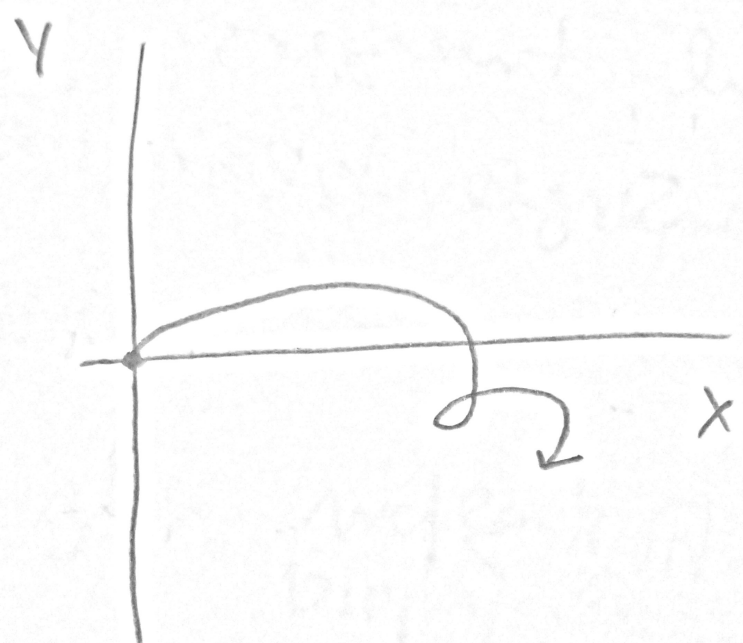
\includegraphics[width=0.5\linewidth]{screenshot003}
			\end{center}
			
		\end{enumerate}
	
		\item We can parameterize the loop's $\dd{\bvec{l}}$ with an angle $\theta$, \begin{align*}
			y & = a\cos \theta \\
			\dd{y} & = -a\sin \theta \dd{\theta} \\
			z & = a\sin \theta \\
			\dd{z} & = a\cos \theta \dd{\theta} \\
			\dd{\bvec{l}} & = -a\sin \theta \dd{\theta} \uvec{y} + a\cos \theta \uvec{z} \dd{\theta}
			\intertext{Crossing this with $\bvec{B}$,}
			\dd{\ell} \cross \bvec{B} & = - kz^2 a \cos \theta \dd{\theta} \uvec{y} - kz^2 a \sin \theta \dd{\theta} \uvec{z} \\
				& = -k a \sin[2](\theta) \left( \cos \theta \uvec{y} + \sin \theta \uvec{z} \right) \dd{\theta}
			\intertext{The force can be found by integrating from $0$ to $2\pi$,}
			\bvec{F} & = -kIa \int_{0}^{2 \pi} \sin[2](\theta)\left( \cos \theta \uvec{y} + \sin \theta \uvec{z} \right) \dd{\theta} \\
				& = 0?
		\end{align*}
		\item The uniform charge density is \begin{align*}
			\rho & = \frac{Q}{V} = \frac{3Q}{4 \pi R^3}
			\intertext{At any point, the instantaneous velocity is }
			\bvec{v} & = r \uvec{\phi}
			\intertext{The volume current density is then}
			\bvec{J} & = \rho \bvec{v} \\
				& = \frac{3Q r}{4 \pi R^3} \uvec{\phi}
		\end{align*}
	
		\item \begin{enumerate}
			\item Using Example 5.5 as a starting point, we can use the angles \begin{align*}
				\theta_1 & = -\pi/4 \\
				\theta_2 & = \pi / 4
				\intertext{And use equation (5.37)}
				\bvec{B} & = \frac{\mu_0 I}{4 \pi d} \sqrt{2} \text{ (out of page)}
			\end{align*}
		
			\item Here, there's a constant radius $R$, so the Biot-Savart law simplifies \begin{align*}
				\bvec{B} & = \frac{\mu I}{4 \pi} \left(\pi R / R^2\right) \\
					& = \frac{\mu I}{4 R } \text{ (into page)}
			\end{align*}
		\end{enumerate}
	
		\item We can just integrate over the the length of the cylinder, where $z$ now goes from $-L/2$ to $L/2$, and the current $I = \lambda (R \omega)$, \begin{align*}
			B & = \frac{\mu_0 \lambda \omega R^3}{2} \int_{-L/2}^{L/2} (R^2 + z^2)^{-3/2} \dd{z} \\
			\bvec{B} & = \frac{\mu_0 \lambda \omega R^2 L}{\sqrt{L^2 + 4R^2}} \uvec{z} \quad \text{ (WolframAlpha)}
			\intertext{As $L$ tends to infinity, it'll approach a constant}
			\bvec{B} & = {\mu_0 \lambda \omega R^2} \uvec{z}
		\end{align*}
	\end{enumerate}
\end{document}